%%%%%%%%%%%%%%%%%%%%%%%%%%%%%%%%%%%%%%%%%%%%%%%%%%%%%%%%%%
%%
%% The Title
%%
%%%%%%%%%%%%%%%%%%%%%%%%%%%%%%%%%%%%%%%%%%%%%%%%%%%%%%%%%%

\chapter*{\S B28. Diffeological Spaces are Locally Connected}
\setcounter{footnote}{0}

%%%%%%%%%%%%%%%%%%%%%%%%%%%%%%%%%%%%%%%%%%%%%%%%%%%%%%%%%%
%%
%% MARK: Abstract
%%
%%%%%%%%%%%%%%%%%%%%%%%%%%%%%%%%%%%%%%%%%%%%%%%%%%%%%%%%%%

\begin{abstract}
  Something that should have been said a long time ago:
  Every diffeological space is locally connected for the D-topology.
\end{abstract}

Let us recall that every diffeological space $X$ naturally carries a topology called the D-topology.
It was defined originally in \cite{Igl85} but see also \cite[\textsection\,2.8]{PIZ13}.
It is the finest topology for which the plots are continuous.
A subset $\cO \subset X$ is open for the D-topology,
or is \emph{D-open},
if $P^{-1}(\cO)$ is open in $\Domain(P)$ for all plots $P$ in $X$.

It has been shown that the connected components for the D-topology are the path-connected components,
and that the space $X$ is the sum of its connected components \cite[\textsection\,5.7, 5.8]{PIZ13}.

We can say more about that,
but first we recall one of the definitions of \emph{locally connected spaces}.

\begin{Article}{Definition.}{\itshape
  A topological space is said to be \emph{locally connected} if every open subset is the sum of its components
  for the induced topology.
}
\end{Article}

Then:

\begin{Article}{Proposition.}{\itshape
  Every diffeological space is locally connected.
  That is,
  every D-open subset $\cO$ is the sum of its connected components for the D-topology induced on $\cO$.
  Since connected components for the D-topology coincide with pathwise connected components,
  every connected diffeological space is locally pathwise connected.
}
\end{Article}

\begin{proof}
  Let us prove that D-open subsets $\cO \subset X$ are embedded \cite[\textsection\,2.14]{PIZ13}.
  That is,
  every D-open subset $\cU$ of the subspace $\cO \hookrightarrow X$ is the imprint of a D-open subset $\cU'$ of $X$,
  \emph{i.e.},
  $$
    \cU = \cU' \cap \cO,
  $$
  where $\cU'$ is D-open in $X$ and $\cU$ is D-open in $\cO$ for its D-topology as a subspace.
  
  On the one hand,
  since $\cU$ is open for the D-topology of the subspace $\cO$ of $X$,
  then for every plot $P$ in $\cO$,
  that is,
  for every plot $P$ in $X$ taking its values in $\cO$,
  $P^{-1}(\cU)$ is open.
  
  On the other hand,
  let $P$ be any plot in $X$.
  Since $P^{-1}(\cU) \subset P^{-1}(\cO)$,
  we have $P^{-1}(\cU) = [P\restriction P^{-1}(\cO)]^{-1}(\cU)$.
  But $P^{-1}(\cO)$ is open because $\cO$ is D-open,
  so $P\restriction P^{-1}(\cO)$ is still a plot in $X$ taking its values in $\cO$,
  hence a plot in $\cO$.
  Thus $[P\restriction P^{-1}(\cO)]^{-1}(\cU)$ is open,
  and therefore $P^{-1}(\cU)$ is open.
  Hence,
  for all plots $P$ in $X$,
  $P^{-1}(\cU)$ is open.
  Consequently,
  $\cU$ is D-open in $X$,
  and since $\cU = \cU \cap \cO$,
  $\cU$ as a D-open subset of $\cO$ is the imprint of $\cU$ (which is D-open in $X$) on $\cO$.
  In conclusion,
  every D-open subset of $X$ is embedded.
  
  In summary,
  the relation $\cU = \cU' \cap \cO$ above reads as follows:
  every D-open subset of $\cO$ is D-open in $X$,
  since it is the intersection of two D-open subsets of $X$ (namely $\cU$ itself and $\cO$).
  
  Now,
  as a subspace of $X$,
  $\cO$ is the sum of its components,
  which are D-open subsets of $\cO$,
  and therefore D-open subsets of $X$ as well.
  Thus $\cO$ is the sum of its components for the D-topology of $X$.
  Therefore $X$ is locally connected for the D-topology.
\end{proof}

\vfill
\centerline{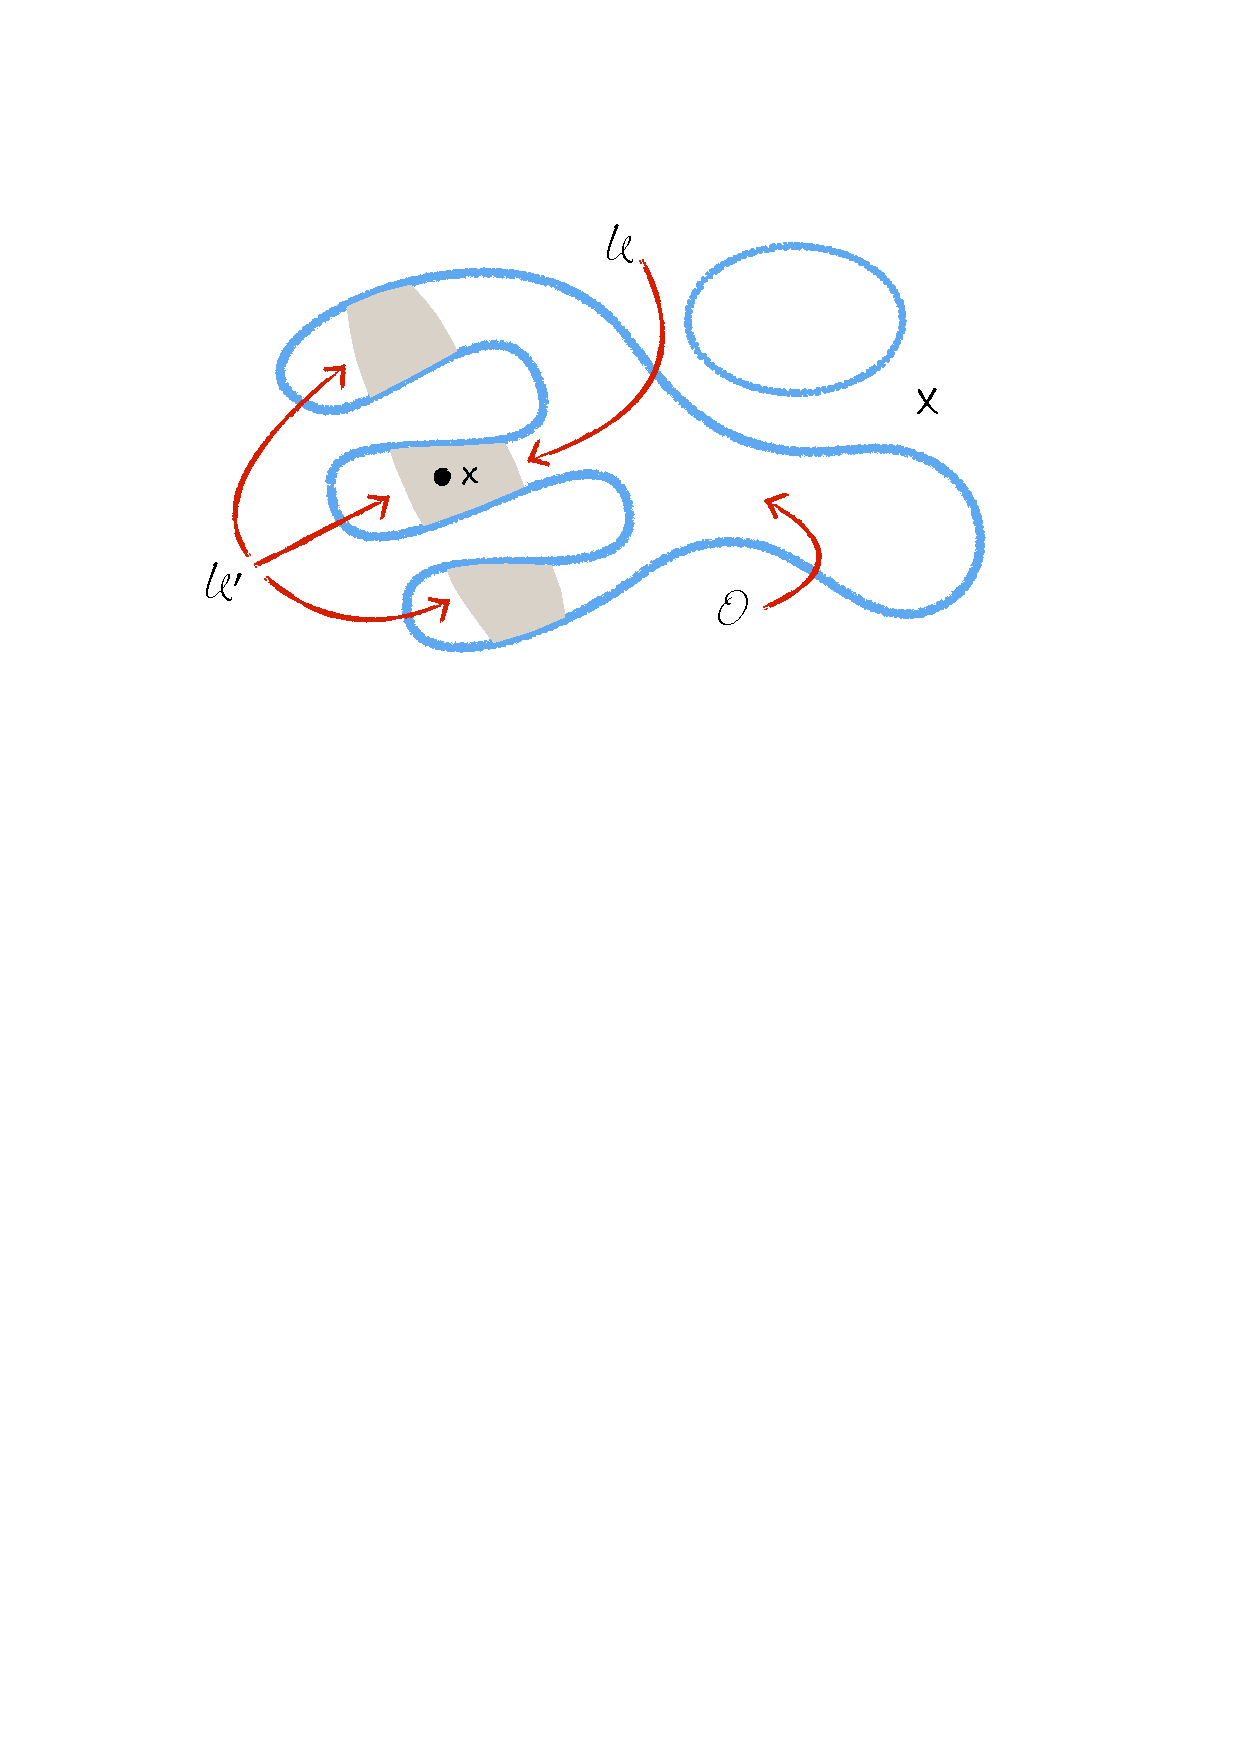
\includegraphics[width=.65\textwidth]{Figures/Locally-connected.pdf}}
